\documentclass{article}
\usepackage[utf8]{inputenc}
\usepackage{listings}
\usepackage{xcolor}
\usepackage{graphicx}
\graphicspath{ {images/} }
\usepackage{amsmath}
\usepackage{float}
\documentclass{article}
\usepackage[utf8]{inputenc}
\usepackage{listings}
\usepackage{xcolor}
\usepackage{graphicx}
\graphicspath{ {images/} }

%New colors defined below
\definecolor{codegreen}{rgb}{0,0.6,0}
\definecolor{codegray}{rgb}{0.5,0.5,0.5}
\definecolor{codepurple}{rgb}{0.58,0,0.82}
\definecolor{backcolour}{rgb}{0.95,0.95,0.92}

%Code listing style named "mystyle"
\lstdefinestyle{mystyle}{
  backgroundcolor=\color{backcolour},   commentstyle=\color{codegreen},
  keywordstyle=\color{magenta},
  numberstyle=\tiny\color{codegray},
  stringstyle=\color{codepurple},
  basicstyle=\ttfamily\footnotesize,
  breakatwhitespace=false,         
  breaklines=true,                 
  captionpos=b,                    
  keepspaces=true,                 
  numbers=left,                    
  numbersep=5pt,                  
  showspaces=false,                
  showstringspaces=false,
  showtabs=false,                  
  tabsize=2
}

%"mystyle" code listing set
\lstset{style=mystyle}


\title{BTH004 - Laboratory assignment 2------\\
Theoretical analysis and Practical analysis between merge sort and bubble sort}
\author{name: Zhao Shui--\\student ID: 201806150329}
\date{November 2020}

\begin{document}
\maketitle

\section{description of two algorithm}
\subsection{merge sort}
Use the divide-and-conquer algorithm. divide the original array into two parts, and for each parts redo this action until it can't be divided. and it become n parts(n is the size of the array), and then continuously combine the n parts number in order to the original size.
\subsection{bubble sort}
Use two for loop, it iteratively visit the element of the array to be sorted, compare the two adjacent element in turn. If these two elements are in the wrong order then swap them.

\section{pseudo code for two algorithm}
\subsection{merge sort}
\lstinputlisting[language=Python]{merge.py}
\subsection{bubble sort}
\lstinputlisting[language=Python]{bubble.py}

\section{code for the experiment}
\lstinputlisting[language=Python]{code.py}

\section{theoretical analysis}
\subsection{merge sort}
the number of merge sort is:
\[
f(n) = n\log{n} - n + 1
\]
\subsection{bubble sort}
the number of bubble sort is:
\[
f(n) = \frac{(n-1)n}{2}
\]

\section{theoretical analysis}
\subsection{merge sort}
\begin{figure}[H]
    \centering
    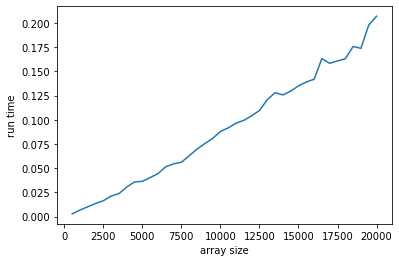
\includegraphics[scale=0.7]{mergeresult1.png}
    \caption{time of merge sort at different size of array}
\end{figure}
\subsection{bubble sort}
\begin{figure}[H]
    \centering
    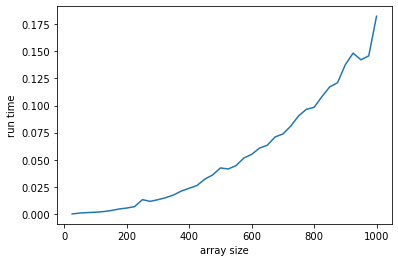
\includegraphics[scale=0.7]{bubbleresult1.png}
    \caption{time of bubble sort at different size of array}
\end{figure}
\section{initialization time at difference array size}
\subsection{merge sort}
\begin{figure}[H]
    \centering
    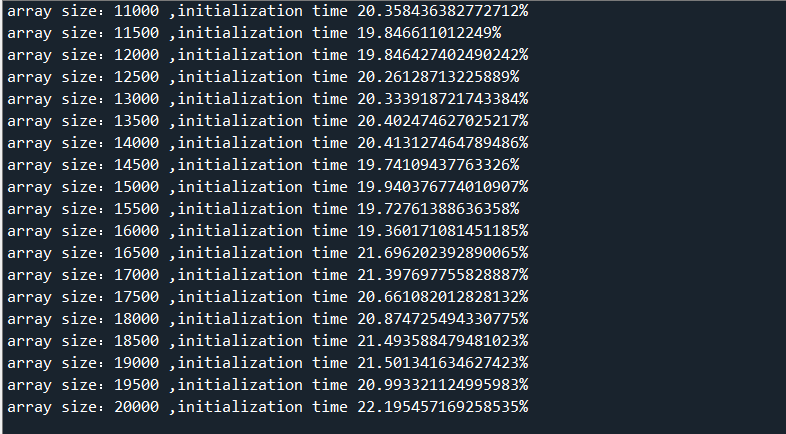
\includegraphics[scale=0.5]{mergetime1.png}
    \caption{initialization time at different size of array}
\end{figure}
And we can find that it almost doesn't have any change when array size changed.
\subsection{bubble sort}
\begin{figure}[H]
    \centering
    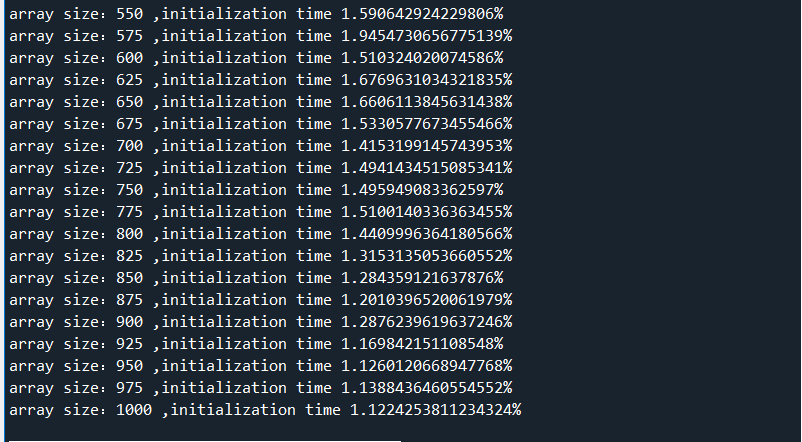
\includegraphics[scale=0.5]{bubbletime1.png}
    \caption{initialization time at different size of array}
\end{figure}
And we can obviously find that when array size increasing, initialization time is decreasing. And when array size come to 1000 or larger, the time is only 1\%.
\begin{figure}[H]
    \centering
    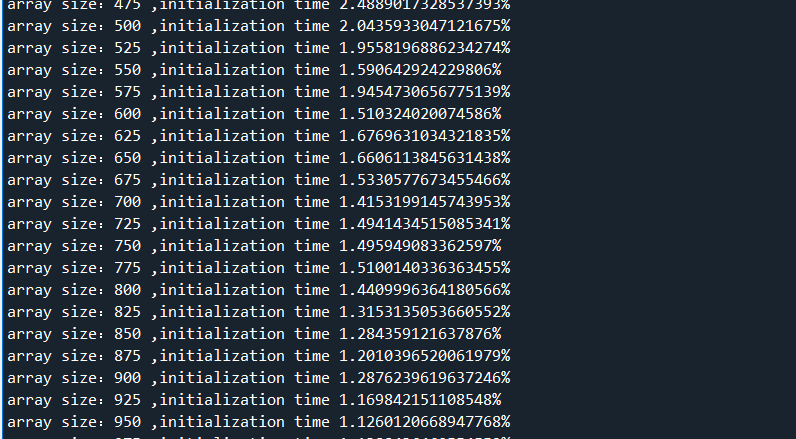
\includegraphics[scale=0.5]{bubbletime2.png}
    \caption{initialization time at different size of array}
\end{figure}
\section{the comparison C of practical and theoretical analyses}
\subsection{merge sort}
\begin{figure}[H]
    \centering
    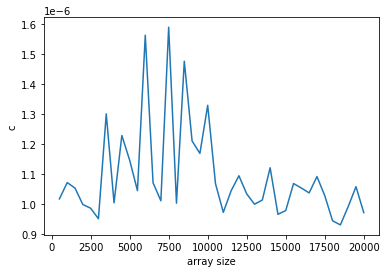
\includegraphics[scale=0.7]{mergeresult2.png}
    \caption{C of merge sort at different size of array}
\end{figure}
\subsection{bubble sort}
\begin{figure}[H]
    \centering
    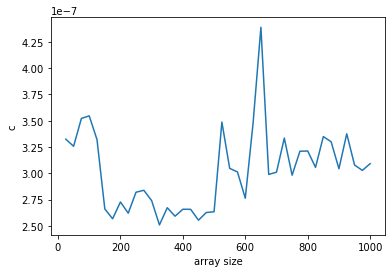
\includegraphics[scale=0.7]{bubbleresult2.png}
    \caption{C of bubble sort at different size of array}
\end{figure}
\end{document}
